

\chapter{CONSTRUCTING AND SHEARING ICE-I$_\mathrm{h}$ / WATER INTERFACES}

\begin{flushright}
\textit{''Why do snowflakes always fall as flat structures with six corners?''} \\
-Joannes Kepler (1611) \\
\end{flushright}


Non-equilibrium molecular dynamics simulations of solid / liquid
friction at the basal $\{0001\}$, prismatic $\{10\bar{1}0\}$,
14\degree~pyramidal $\{20\bar{2}1\}$, and secondary prism
$\{11\bar{2}0\}$ facets of an ice-I$_\mathrm{h}$ crystal were
performed. Contained in this chapter are the details of how these
systems were constructed as well as the computational details
of the simulations. In addition, non-equilibrium molecular dynamics
methodologies and water models are discussed.


\section{Construction of Ice-I$_\mathrm{h}$ / Water Interfaces}

Ice-I$_\mathrm{h}$ crystallizes in the hexagonal space group
P$6_3/mmc$, and ice crystals normally form hexagonal plates with the
basal face, $\{0001\}$, forming the top and bottom of each plate, and
the prismatic facet, $\{10\bar{1}0\}$, forming the sides.  In extreme
temperatures or low water saturation conditions, ice crystals can form
hollow columns, needles, and dendrites, exposing other crystalline
facets of the ice to the surroundings.  Among the more
commonly-observed facets are the secondary prism, $\{11\bar{2}0\}$,
and the two pyramidal, 14\degree~$\{20\bar{2}1\}$ and
28\degree~$\{10\bar{1}1\}$, faces. Images of these surfaces can
be found in Fig. \ref{fig:surfMorph}.


\begin{figure} 
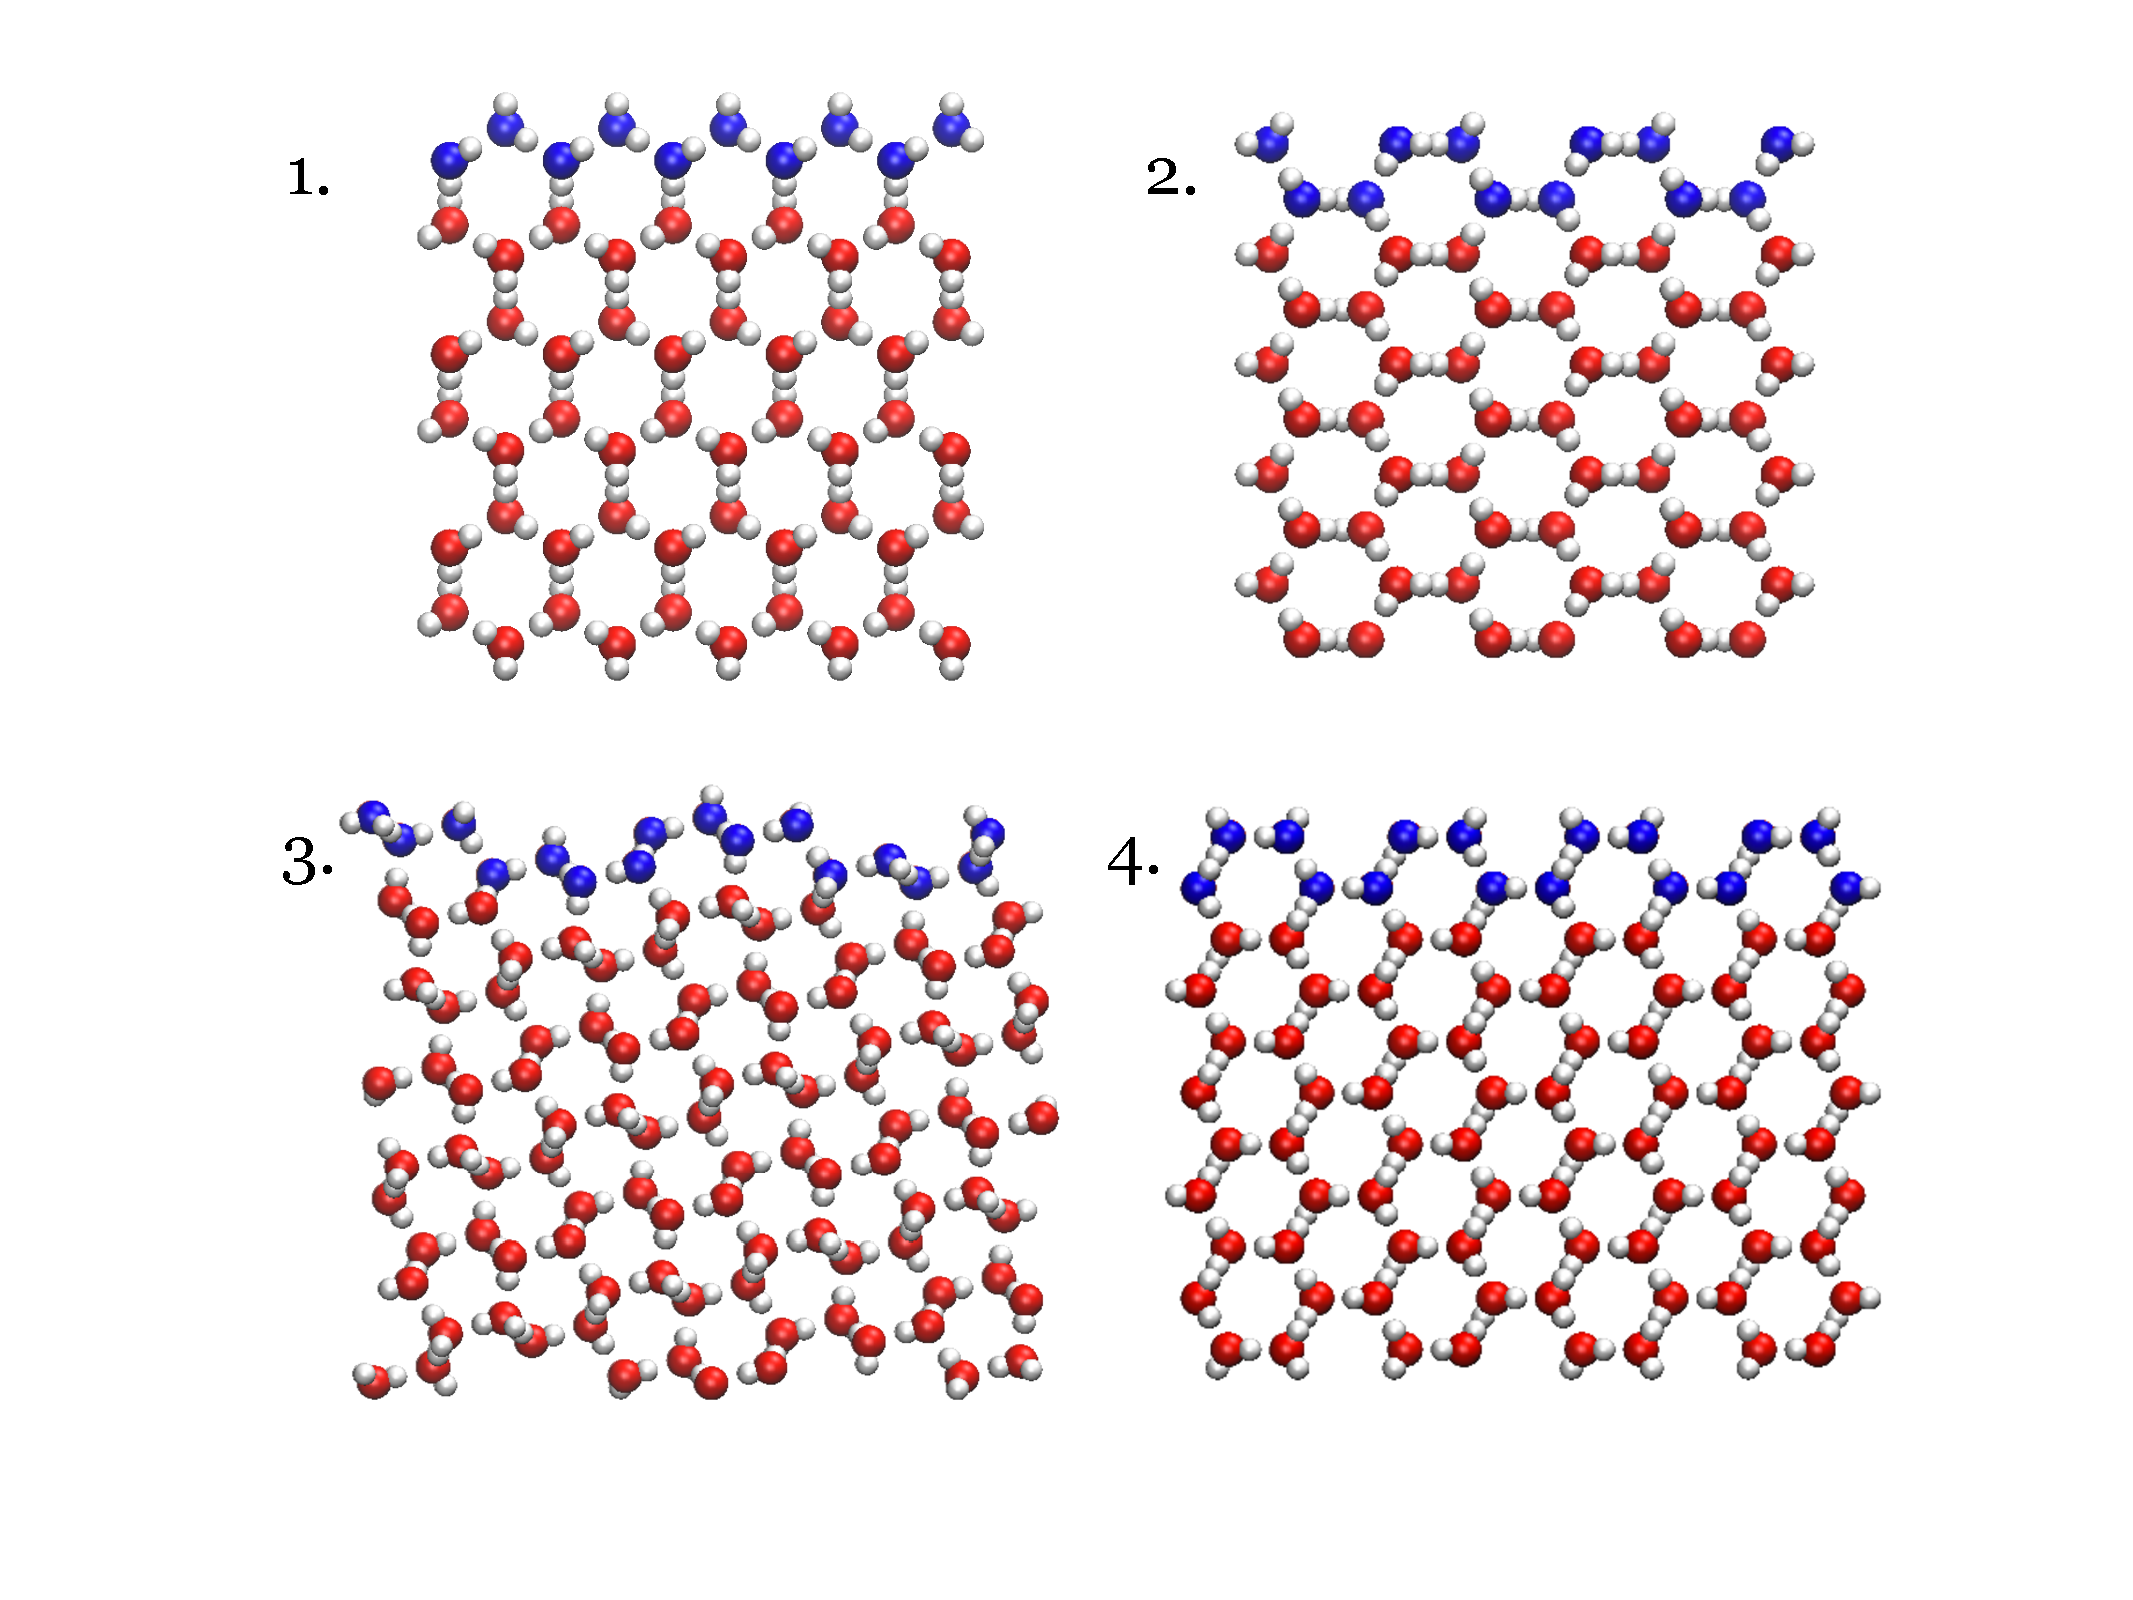
\includegraphics[width=1.0\linewidth]{Figures/surfMorph}
\caption{\label{fig:surfMorph}The basal (1), prismatic (2),
  14\degree~pyramidal (3), and secondary prism (4) facets of an
  ice-I$_\mathrm{h}$ crystal, generated by replication of unit cell
  structure 6 by Hirsch and Ojam\"{a}e. Left column and middle column:
  the two perpindicular side-on views of the crystal facet. Right
  column: looking down on the crystal face (the 14\degree~pyramidal
  surface has been tilted to better observe the surface). The surface oxygens have
  been colored blue for clarity.}
\end{figure}

Surface energies, dimensions of crystal channels at zero kelvin, ...

The oxygen lattice is a hexagonal unit cell comprising 4 oxygen atoms,
but it is also possible to construct an equivalent orthorhombic unit
cell with 8 oxygen atoms.\cite{Hirsch2004} Hydrogen atom placement
obeys the Bernal-Fowler ice rules which distribute protons so that
each oxygen donates two hydrogen bonds and accepts two from
neighboring molecules.\cite{Bernal1933} The resulting structure also
typically has zero net dipole moment. Below 72~K and under ambient
pressures, the lattice can undergo a phase transition to ice-XI, a
configuration with ferroelectric proton-ordering and a non-zero bulk
dipole moment (see Fig. \ref{fig:iceTransition}).

\begin{figure} 
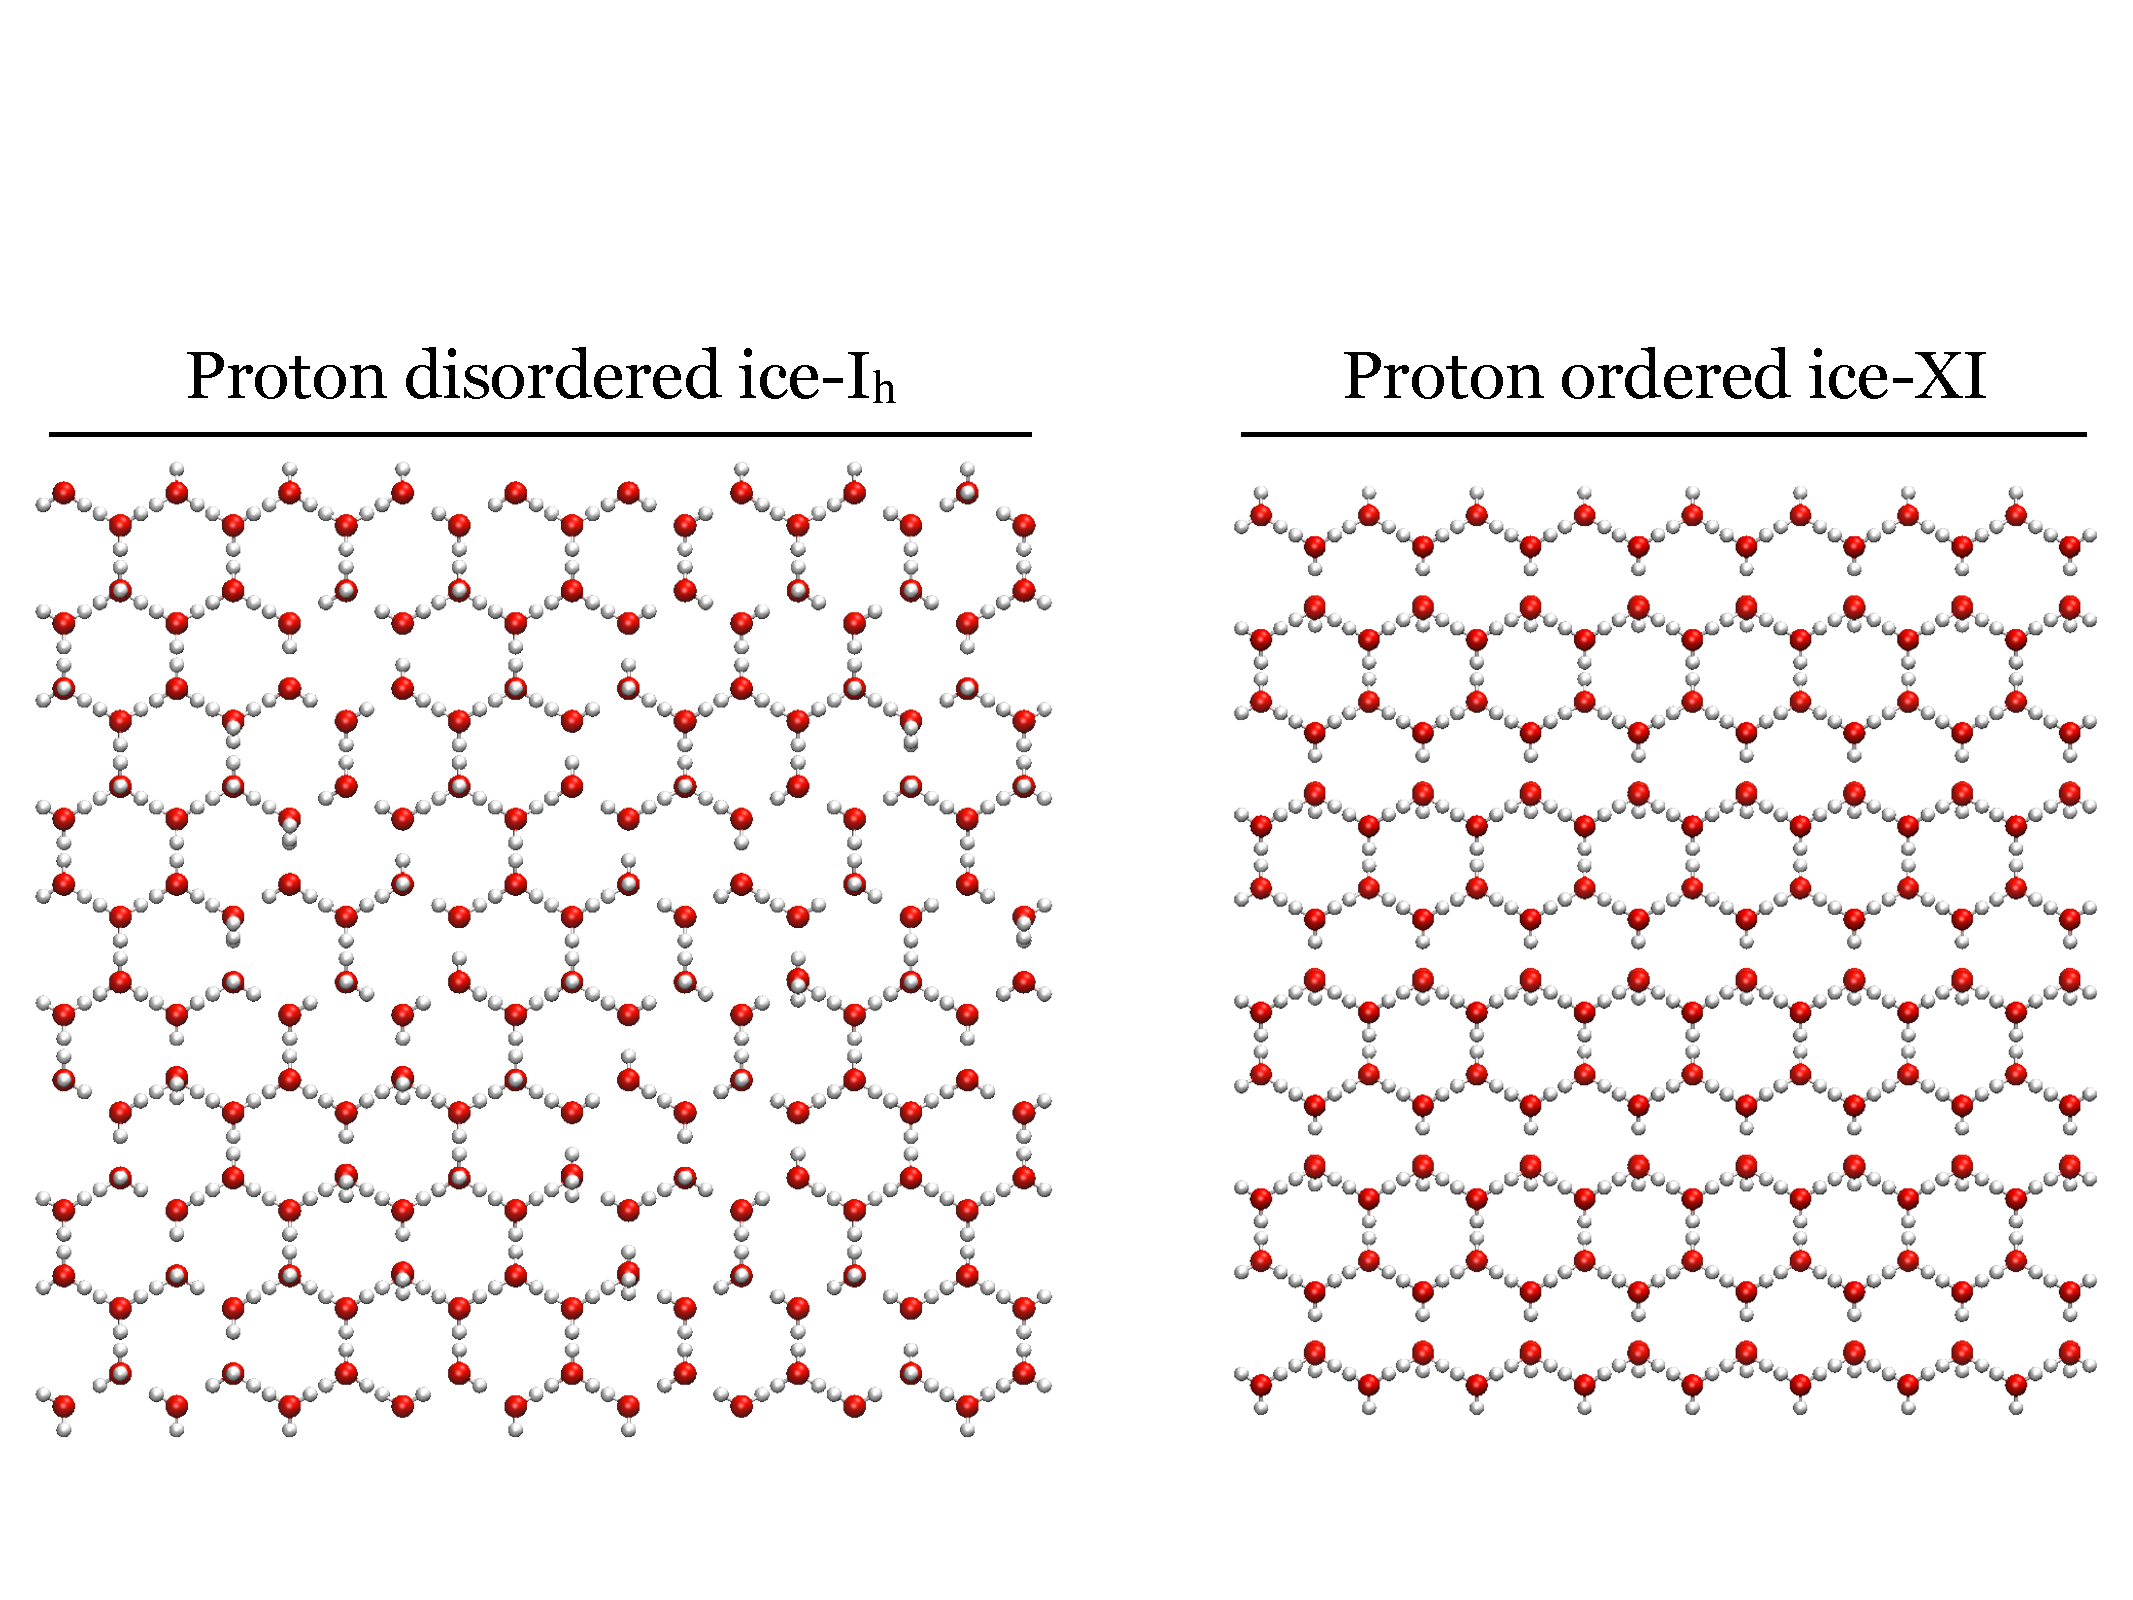
\includegraphics[width=\linewidth]{Figures/iceTransition}
\caption{\label{fig:iceTransition}Left: A proton-disordered
  ice-I$_\mathrm{h}$ crystal (zero-net dipole moment), viewed down
  onto the basal facet. Coordinates for this crystal structure are
  taken from Hayward and Reimers.\cite{Hayward1997} Right: A
  proton-ordered ice-XI crystal (non-zero net dipole moment), viewed
  down on the same crystal face. Coordinates for this structure are
  taken from Structure 1 of Hirsch and Ojam\"{a}e.\cite{Hirsch2004}
  The phase transition between ice-I$_\mathrm{h}$ and ice-XI is
  believed to be $\sim$ 72~K.}
\end{figure}

While exploring the ice-I$_\mathrm{h}$ to ice-XI phase transition, Hirsch
and Ojam\"{a}e determined sixteen unique hydrogen arrangements for the
ice-I$_\mathrm{h}$ orthorhombic unit cells.\cite{Hirsch2004} Upon
replication of some of these unit cells, the resulting structures
present stripes of dangling H-atoms and lone pairs at an exposed
crystal facet. These orthorhombic initial configurations can be used
to reproduce the surface features from Buch \textit{et
  al.}\cite{Buch2008} that helped interpret sum-frequency generation
(SFG) experiments by the Shultz lab.\cite{Groenzin2007} More recently,
Nojima \textit{et al.}\cite{Nojima2017} have successfully obtained
both the real and imaginary parts of the vibrational spectra of the
free OH stretch for surface water molecules of the basal, prismatic,
and secondary prismatic facets at ca. 130~K through
heterodyne-detected sum-frequency generation (HD-SFG). They also
present evidence of proton-striped surfaces as the sign of the
imaginary part of the vibrational spectra indicates ``up'' or ``down''
orientations of surface molecules.

\begin{table}
\centering
  \caption{MAPPING BETWEEN THE MILLER INDICES OF FOUR FACETS OF ICE IN
    THE $P6_3/mmc$ CRYSTAL SYSTEM TO THE ORTHORHOMBIC $P2_12_12_1$
    SYSTEM IN REFERENCE \bibpunct{}{}{,}{n}{}{,} \protect\citep{Hirsch04}.}
\label{tab:equiv}
\begin{tabular}{|ccc|} \hline
 & hexagonal & orthorhombic \\
 & ($P6_3/mmc$) & ($P2_12_12_1$) \\
 crystal face  & Miller indices & equivalent \\ \hline
basal & $\{0~0~0~1\}$ & $\{0~0~1\}$ \\
prism & $\{1~0~\bar{1}~0\}$ & $\{1~0~0\}$ \\
secondary prism & $\{1~1~\bar{2}~0\}$ & $\{1~3~0\}$ \\
pyramidal & $\{2~0~\bar{2}~1\}$ & $\{2~0~1\}$ \\ \hline
\end{tabular}
\end{table}

SPC/E~\cite{Berendsen1987} and TIP4P/Ice~\cite{Abascal2005} structures
were created starting from Structure 6 of Hirsch and Ojam\"{a}e's set
of orthorhombic representations for ice-I$_{h}$.\cite{Hirsch2004}
Replication of Structure 6 (unit cell geometry $P2_12_12_1$) produces
a proton-ordered version of ice-I$_\mathrm{h}$ on a smaller length
scale than the simulation box. However, the resulting crystal has a
zero-net dipole, unlike proton ordered ice-XI crystals.  Structure 6
from the Hirsch and Ojam\"{a}e paper has lattice parameters
$a = 4.49225$ \AA\ , $b = 7.78080$ \AA\ , $c = 7.33581$ \AA\ and two
water molecules whose atoms reside at fractional coordinates given in
Table \ref{tab:p212121}.  Table \ref{tab:equiv} contains a mapping
between the Miller indices of common ice facets in the P$6_3/mmc$
crystal system and those in the Hirsch and Ojam\"{a}e $P2_12_12_1$
system.

\begin{table}
\centering
  \caption{FRACTIONAL COORDINATES FOR WATER IN THE ORTHORHOMBIC
    $P2_12_12_1$ SYSTEM FOR ICE I$_\mathrm{h}$ IN REFERENCE \bibpunct{}{}{,}{n}{}{,} \protect\citep{Hirsch0404}.}
\label{tab:p212121}
\begin{tabular}{|cccc|}  \hline
atom type & x & y & z \\ \hline
 O & 0.7500 & 0.1667 & 0.4375 \\
 H & 0.5735 & 0.2202 & 0.4836 \\
 H & 0.7420 & 0.0517 & 0.4836 \\
 O & 0.2500 & 0.6667 & 0.4375 \\
 H & 0.2580 & 0.6693 & 0.3071 \\
 H & 0.4265 & 0.7255 & 0.4756 \\ \hline
\end{tabular}
\end{table}


In order to generate large crystals for simulation, the primitive unit
cell was replicated in all dimensions. The crystal was cleaved along
the desired face, and two additional mutually perpendicular cuts were
made.  The crystal was reoriented so that the initial cut (basal,
prismatic, 14 \degree~pyramidal, or secondary prism) was normal to the
$z$-axis of the simulation cell.  The resulting structures were
extended in $x$ and $y$ to form large exposed facets in rectangular
box geometries.  Because the orthorhombic unit cells are relatively
small, using these as building blocks for an ice simulation creates
proton translational order on the length scale of the unit cells. We
note that all simulated ice structures have proton ordering on the
length scale of the periodic box, but in order to reproduce proton
surface striping with zero dipole crystals, we have utilized proton
translational ordering on a smaller length scale than other ice
studies.

Liquid water boxes were created with identical dimensions (in $x$ and
$y$) as the ice, with a $z$ dimension of three times that of the ice
block, and with a density corresponding to $1$ g / cm$^3$.  Each of
the ice slabs and water boxes were independently equilibrated to
$50$~K and a pressure of $1$ atm by coupling the temperature and
pressure of the system to a heat and pressure bath. The resulting
systems were merged by carving out any liquid water molecules within
3~\AA~ of any atoms in the ice slabs.  For the SPC/E simulations, the
combined ice / water systems were equilibrated to 225~K. The
liquid-ice coexistence temperature for SPC/E water has been reported
as $215 \pm 4$~K.\cite{Vega2006a,Fernandez2006} We observed a
coexistence temperature of 225~K for our crystals, possibly due to the
surface striped structures utilized in this study. For the TIP4P/Ice
simulations, the combined ice / water system was equilibrated to the
reported coexistence temperature, 270~K.\cite{Vega2006a,Fernandez2006}
The quiescent ice / water interfaces were then equilibrated for 10 ns,
with 5 ns under a constant temperature (NVT) integrator, followed by 5
ns under a microcanonical (NVE) integrator.  During this time the ice
was monitored for crystal growth or melting. We observed no advance of
the ice interface into the liquid, and no loss of crystallinity of the
ice. The resulting dimensions as well as the number of ice and liquid
water molecules contained in each of these systems are shown in Table
\ref{tab:sizes}.  Note that the water molecules are not restrained in
any way - molecules that start in the liquid phase may exchange with
the ice (and vice versa).

\begin{table}
\centering
\caption{SIZES OF THE ICE / WATER SHEARING SIMULATIONS. (Box
  dimensions are given in \AA)\label{tab:sizes}}
\begin{tabular}{r|cc|ccc|ccc}
\toprule
 & & & \multicolumn{3}{c|}{SPC/E~(225~K)} &  \multicolumn{3}{c}{TIP4P/Ice~(270~K)}\\
 Interface & $N_\mathrm{ice}$ &
 $N_\mathrm{liquid}$ & $L_x$ & $L_y$ & $L_z$ & $L_x$ & $L_y$ & $L_z$ \\
\midrule
Basal  $\{0001\}$                 & 900 & 1846  & 23.87 & 35.83 & 98.64  & 23.37 & 38.83 & 97.67  \\
Prismatic  $\{10\bar{1}0\}$       & 3000 & 5464 & 35.95 & 35.65 & 205.77 & 36.33 & 38.86 & 191.75 \\
14 \degree~Pyramidal  $\{20\bar{2}1\}$       & 1216 & 2203 & 37.47 & 29.50 & 93.02  & 37.16 & 30.19 & 97.65  \\
Secondary Prism  $\{11\bar{2}0\}$ & 3840 & 8176 & 71.87 & 31.66 & 161.55 & 72.90 & 32.06 & 165.17 \\
\bottomrule
\end{tabular}
\end{table}


The liquid-state viscosity of the SPC/E water model has been
extensively characterized over a wide range of liquid
conditions~\cite{Kuang2012}, and its phase diagram has been well
studied~\cite{Baez1995,Bryk2004,Sanz2004a,Fennell2005}. With longer
cutoff radii and careful treatment of electrostatics, SPC/E mostly
avoids metastable crystalline morphologies like
ice-\textit{i}~\cite{Fennell2005} and ice-B~\cite{Baez1995}, although
Sanz \textit{et al.}\cite{Sanz2004a} found that the stable polymorph
for this model is likely ice-II at this temperature and 1 bar. The
free energies and melting
points~\cite{Baez1995,Arbuckle2002,Gay2002,Bryk2002,Bryk2004,Sanz2004a,Fennell2005,Fernandez2006,Abascal2007,Vrbka2007}
of various other crystalline polymorphs have also been calculated.
Haymet \textit{et al.}\cite{Bryk2002} have studied quiescent
ice-I$_\mathrm{h}$ / water interfaces using the SPC/E water model, and
have seen structural and dynamic measurements of the interfacial width
that agree well with both experimental results and more expensive
water models, although the coexistence temperature for SPC/E is still
well below the experimental melting point of real water.  

Recent investigations have questioned the applicability of SPC/E in
ice / water
simulations,\cite{Vega2005c,Vega2011a,Gladich2012,Gallo2016} however,
so simulations have also been done using TIP4P/Ice.\cite{Abascal2005}
This model was parameterized by fitting the equation of state, as well
as the melting and coexistence lines involving different
ice polymorphs, and the resulting melting temperature of
ice-I$_\mathrm{h}$ (270~K) is much closer to the experimental
value (273.15~K).\cite{Abascal2005} Although TIP4P/Ice is more computationally
demanding, it is worthwhile to compare models where liquid water is in
contact with ice at multiple coexistence temperatures.

\section{Shearing Ice-I$_\mathrm{h}$ / Water Interfaces Without Bulk Melting}

As a solid is dragged through a liquid, there is frictional heating
that will act to melt the interface.  Close to the melting point of the
solid, this frictional heating may result in melting of the crystal.
We are interested in the structure and dynamics of the interface at
the coexistence temperature.  This can be accomplished using the velocity
shearing and scaling (VSS) variant of reverse non-equilibrium
molecular dynamics (RNEMD), which utilizes a series of simultaneous
velocity exchanges between two regions within the simulation
cell.\cite{Kuang2012} One of these regions is centered within the ice
slab, while the other is centrally located in the liquid
region. VSS-RNEMD provides a set of conservation constraints for
creating either a momentum flux or a thermal flux (or both
simultaneously) between the two slabs.  Satisfying the constraint
equations ensures that the new configurations are sampled from the
same NVE ensemble as before the VSS move.

The VSS moves are applied periodically to scale and shift the particle
velocities ($\mathbf{v}_i$ and $\mathbf{v}_j$) in two slabs ($H$ and
$C$) which are separated by half of the simulation box,
\begin{displaymath}
\begin{array}{rclcl}

 & \underline{\mathrm{shearing}} & &
 \underline{~~~~~~~~~~~~\mathrm{scaling}~~~~~~~~~~~~} \\
\mathbf{v}_i \leftarrow & 
  \mathbf{a}_c\ & + & c\cdot\left(\mathbf{v}_i - \langle\mathbf{v}_c
  \rangle\right)  +  \langle\mathbf{v}_c\rangle \\
\mathbf{v}_j \leftarrow & 
  \mathbf{a}_h & + & h\cdot\left(\mathbf{v}_j - \langle\mathbf{v}_h
    \rangle\right) + \langle\mathbf{v}_h\rangle .

\end{array}
\end{displaymath}
Here $\langle\mathbf{v}_c\rangle$ and $\langle\mathbf{v}_h\rangle$ are
the center of mass velocities in the $C$ and $H$ slabs, respectively.
Within the two slabs, particles receive incremental changes or a
``shear'' to their velocities.  The amount of shear is governed by the
imposed momentum flux, $\mathbf{j}_z(\mathbf{p})$
\begin{eqnarray}
\mathbf{a}_c & = & - \mathbf{j}_z(\mathbf{p}) \Delta t / M_c \label{vss1}\\
\mathbf{a}_h & = & + \mathbf{j}_z(\mathbf{p}) \Delta t / M_h \label{vss2}
\end{eqnarray}
where $M_{\{c,h\}}$ is the total mass of particles within each of the
slabs and $\Delta t$ is the interval between two separate operations.

To simultaneously impose a thermal flux ($J_z$) between the slabs we
use energy conservation constraints,
\begin{eqnarray}
K_c - J_z\Delta t & = & c^2 (K_c - \frac{1}{2}M_c \langle\mathbf{v}_c
\rangle^2) + \frac{1}{2}M_c (\langle \mathbf{v}_c \rangle + \mathbf{a}_c)^2 \label{vss3}\\
K_h + J_z\Delta t & = & h^2 (K_h - \frac{1}{2}M_h \langle\mathbf{v}_h
\rangle^2) + \frac{1}{2}M_h (\langle \mathbf{v}_h \rangle +
\mathbf{a}_h)^2 \label{vss4}.
\label{constraint}
\end{eqnarray}
Simultaneous solution of these quadratic formulae for the scaling
coefficients, $c$ and $h$, will ensure that the simulation samples from
the original microcanonical (NVE) ensemble.  Here $K_{\{c,h\}}$ is the
instantaneous translational kinetic energy of each slab.  At each time
interval, it is a simple matter to solve for $c$, $h$, $\mathbf{a}_c$,
and $\mathbf{a}_h$, subject to the imposed momentum flux,
$j_z(\mathbf{p})$, and thermal flux, $J_z$, values.  Since the VSS
operations do not change the kinetic energy due to orientational
degrees of freedom or the potential energy of a system, configurations
after the VSS move have exactly the same energy (and linear
momentum) as before the move.

As the simulation progresses, the VSS moves are performed on a regular
basis, and the system develops a thermal and/or velocity gradient in
response to the applied flux.  In a bulk material, it is quite simple
to use the slope of the temperature or velocity gradients to obtain
either the thermal conductivity or shear viscosity,
$\eta$.\cite{Bordat2002a}
\begin{equation}
\label{eq:viscosity}
j_z(p_x) = -\eta \left(\frac{\partial v_x}{\partial z}\right).
\end{equation}
At interfaces between dissimilar materials, the same method can be
used to extract \textit{interfacial} transport properties (e.g. the
hydrodynamic slip length or the interfacial thermal
conductance).


The VSS-RNEMD approach is versatile in that it may be used to
implement thermal and shear transport simultaneously.  Perturbations
of velocities away from the ideal Maxwell-Boltzmann distributions are
minimal, as is thermal anisotropy.  This ability to generate
simultaneous thermal and shear fluxes has been previously utilized to
map out the shear viscosity of SPC/E water over a wide range of
temperatures (90~K) with a single 1~ns simulation.\cite{Kuang2012}

% For our work on ice / water interfaces, we began by introducing a
% kinetic energy flux using VSS-RNEMD. Once the thermal gradients had
% stabilized, linear momentum fluxes were imposed coincident with the
% kinetic energy flux. The resulting velocity gradients were allowed to
% stabilize for 1~ns before data collection began. Four successive 1~ns
% simulations were performed for each shear rate (varying from
% $0.5 \rightarrow 10.0~\mathrm{~m~s}^{-1}$) . All atomic configurations
% (positions and velocities) were saved every 1~ps, while statistical
% measures of the system (e.g. temperature, potential energy, total
% energy, and pressure) were sampled every 0.1~ps during the
% simulation. Velocity and thermal profiles (used to compute friction)
% were sampled every 2~fs. Small variations in the measured interfacial
% widths between successive simulations were observed, but there was no
% indication of bulk melting or crystal growth. That is, no large scale
% changes in the positions of the two interfaces were observed during
% the simulations. 

\section{Computational Details}
All simulations were performed using OpenMD,\cite{OOPSE,openmd} with a
time step of 2 fs and periodic boundary conditions in all three
dimensions.  Electrostatics were handled using the damped-shifted
force real-space electrostatic kernel.\cite{Ewald} When applicable,
VSS-RNEMD moves were attempted every time step. This minimized the
magnitude of individual momentum exchanges.  Forcefield parameters for
both water models can be found in Table \ref{tab:waterModels}.

\begin{table}
\centering
\caption{FORCEFIELD PARAMETERS FOR THE SPC/E AND TIP4P/Ice WATER MODELS.}
\label{tab:waterModels}
\begin{tabular}{|l|c|c|c|c|c|c|c|c|} 
\hline
  Model &  $\sigma$ (\AA) & $\epsilon$ (kJ $\mathrm{mol}^{-2}$) &
                                                              $\mathrm{l}_{1}$
                                                              (\AA) &
                                                                    $\mathrm{l}_{2}$
                                                                      (\AA)
  & $\mathrm{q}_{1}$ (e) & $\mathrm{q}_{2}$ (e) & $\theta$
                                                  ($^{\mathrm{o}}$) &
                                                                      $\phi$ ($^{\mathrm{o}}$) \\ \hline
  SPC/E & 3.166 & 0.650 & 1.000 & - & +0.4238 & -0.8476 & 109.47 & - \\
  TIP4P/Ice & 3.1668 & 0.8822 & 0.9572 & 0.1577 & +0.5897 & -1.1794 &
  104.52 & 52.26 \\
\hline
\end{tabular}
\end {table}


The interfaces were equilibrated for a total of 10 ns at equilibrium
conditions before being exposed to either a shear or thermal gradient.
This consisted of 5 ns under a constant temperature (NVT) integrator
set to 225~K followed by 5 ns under a microcanonical integrator.  Weak
thermal gradients were allowed to develop using the VSS-RNEMD (NVE)
integrator using a small thermal flux ($-2.0\times 10^{-6}$
kcal/mol/\AA$^2$/fs) for a duration of 5 ns to allow the gradient to
stabilize.  The resulting thermal gradients ($< 10$~K over the length
of the simulation box) were allowed to stabilize for 5 ns, and were
found to be sufficient to keep the interface within $\pm 5$ K of the
target temperature (225~K for SPC/E and 270~K for TIP4P/Ice) during
all shearing simulations.

Velocity gradients were then imposed using the VSS-RNEMD (NVE)
integrator with a range of momentum fluxes.  Four successive 1~ns
simulations were performed for each shear rate (varying from
$0.5 \rightarrow 10.0~\mathrm{~m~s}^{-1}$) . All atomic configurations
(positions and velocities) were saved every 1~ps, while statistical
measures of the system (e.g. temperature, potential energy, total
energy, and pressure) were sampled every 0.1~ps during the
simulation. Velocity and thermal profiles (used to compute friction)
were sampled every 2~fs. Small variations in the measured interfacial
widths between successive simulations were observed, but there was no
indication of bulk melting or crystal growth. That is, no large scale
changes in the positions of the two interfaces were observed during
the simulations.  A representative configuration of the solvated
prismatic facet being sheared through liquid water is shown in Figure
\ref{fig:Shearing}.


\begin{figure} 
\includegraphics[width=1.7in]{Figures/Shearing}
\caption{\label{fig:Shearing} Computational model of a slab of ice
  being sheared through liquid water.  The ice presents two copies of
  the prismatic $\{10\bar{1}0\}$ facet towards the liquid phase.  The
  RNEMD simulation exchanges both linear momentum (indicated with
  arrows) and kinetic energy between the central box and the box that
  spans the cell boundary.  The system responds with weak thermal
  gradient and a velocity profile that shears the ice relative to the
  surrounding liquid.}
\end{figure}